\documentclass[12 pt]{scrartcl}
\usepackage{setspace}
\onehalfspacing
\usepackage{amsmath,amssymb,amsfonts,amsthm,mathtools}
\usepackage[english]{babel}
\usepackage[T1]{fontenc}
\usepackage[utf8x]{inputenc}
\usepackage{lmodern}
\usepackage{dsfont}
\usepackage{bbm}
\usepackage[round]{natbib}
\usepackage{color} 
\usepackage[defaultlines=2,all]{nowidow}
\usepackage{caption}
\usepackage[labelformat=simple]{subcaption}
\renewcommand\thesubfigure{(\alph{subfigure})}

\setlength\parindent{0pt}
\setlength{\parskip}{6pt plus 1pt minus 1pt}

\newcommand{\red}{\textcolor{red}}


\begin{document}
	
	
	
	\begin{titlepage}
		\centering
		{\scshape\LARGE TU Dortmund \par}
		\vspace{1cm}
		{\scshape\Large Seminar \par}
		\vspace{2cm}
		{\huge\bfseries Model Averaging\par}
		\vspace{2cm}
		{\Large Lecturers:\\
			Prof.\ Dr. Paul Bürkner\\
			Dr.\ Javier Aguilar\\
			Soham Mukherjee\\ \par}
		\vspace{1cm}
		{\Large Author: Md Ryad Ahmed Biplob \par}
		\vspace{0.5 cm}
		{\Large Group number: 1\par}
		\vspace{0.5 cm}
		{\Large Group members: Sharmin Ahmed}
		\vfill
		{\large \today\par}
	\end{titlepage}
	
	
	
	\tableofcontents
	\thispagestyle{empty}
	
	\cleardoublepage
	
	\setcounter{page}{1}
	
	\section{Introduction}
	
	When faced with a challenge, we often look to create a model to understand and predict the outcome. Consider the scenario of being late for class. The exact amount of time one is late is a result of many contributing factors, and a good model should capture as many of them as possible. For example, one model might focus on how much an individual overslept, using historical data from the alarm clock habits. A second model could emphasize traffic congestion, incorporating real-time data from a mapping service. A third might be a simple function of the car’s mechanical reliability.
	
	Each of these models, when used alone, could give a different prediction for an individual's lateness. The first might say the person will be 10 minutes late, the second says 15, and the third says 5. The problem is, we can never be certain which of these is the "true" model that perfectly captures our specific situation. Choosing just one model and acting on its prediction would be shortsighted and possibly lead to further lateness. If only there were a technique to leverage all of them, to combine their strengths and account for their individual uncertainties. This is precisely the problem that Bayesian Model Averaging (BMA) seeks to solve.
	
	\section{Statistical methods}
	
	\subsection{Bayesian Inference}
	According to \citep[1.1]{BMCP2021}, Bayesian Models have two defining characteristics:
	\begin{itemize}
		\item Unknown quantities, also known as parameters, which are described using probability distributions
		\item The usage of Bayes' Theorem to update the values of the parameters conditioned by the data
	\end{itemize}
	Given some observed sample data $\boldsymbol{Y}$ and the parameter $\boldsymbol{\theta}$,
	\begin{equation}
		p(\boldsymbol{\theta}|\boldsymbol{Y}) = \frac{p(\boldsymbol{Y}|\boldsymbol{\theta}) p(\boldsymbol{\theta})}{p(\boldsymbol{Y})}
		\label{eq:1}
	\end{equation}
	where the likelihood function $p(\boldsymbol{Y} |\boldsymbol{\theta})$ quantifies the relationship between the observed data $\boldsymbol{Y}$ and the unknown parameters $\boldsymbol{\theta}$. The prior distribution $p(\boldsymbol{\theta})$ represents our initial beliefs about these parameters before observing any data. Multiplying the likelihood and the prior yields the posterior distribution $p(\boldsymbol{\theta}|\boldsymbol{Y})$, which represents our updated beliefs about the parameters after observing the data. $p(\boldsymbol{Y})$ is the marginal likelihood and acts as a normalising constant, where $\boldsymbol{\Theta}$ is the set of all possible values of $\boldsymbol{\theta}$.
	\begin{equation}
		p(\boldsymbol{Y}) = \int_{\boldsymbol{\theta} \in \Theta}p(\boldsymbol{Y}|\boldsymbol{\theta})p(\boldsymbol{\theta})d\boldsymbol{\theta}
		\label{eq:2}
	\end{equation}
	In some models, the marginal likelihood can be analytically solved. However in most cases, the numerical computation of the integral involves a high-dimensional integration over a usually complicated and highly variable function \cite[11.7]{BMCP2021}. As a result, in most cases, the marginal likelihood is not generally computed and we see Equation \ref{eq:1} expressed as a proportionality.
	\begin{equation}
		p(\boldsymbol{\theta}|\boldsymbol{Y}) \propto p(\boldsymbol{Y}|\boldsymbol{\theta}) p(\boldsymbol{\theta})
		\label{eq:3}
	\end{equation}
	
	\subsection{Bayesian Model Averaging}
	In Equation \ref{eq:3}, the posterior distribution can be considered combining a model with the data. So in practice, if either bad data or a bad model is chosen then the resulting posterior is a combination of both of these factors. This results in the following updated equation \cite[1.1]{BMCP2021}:
	\begin{equation}
		p(\boldsymbol{\theta}|\boldsymbol{Y},\boldsymbol{M}) \propto p(\boldsymbol{Y}|\boldsymbol{\theta},\boldsymbol{M}) p(\boldsymbol{\theta},\boldsymbol{M})
		\label{eq:4}
	\end{equation}
	The specific model $\boldsymbol{M}$ under consideration is typically viewed as one of many plausible models within a set of candidate models $\mathcal{M} = \boldsymbol{\{M_1, \ldots, M_K}\}$. The standard approach is to select a single "best" model, $\boldsymbol{M^\star}$, based on a goodness-of-fit criterion. This single-model selection ignores the inherent uncertainty in choosing one model over others. A significant issue arises when no single model adequately describes the data or when multiple models exhibit similar performance but produces substantially different predictions. Bayesian Model Averaging (BMA) addresses this by computing a marginal distribution—a mixture of the posterior distributions under each $\boldsymbol{M_K}$—where the contribution of each model is weighted by its posterior model probability \cite[p. 383-384]{BMA-Hoeting}. According to \citep{BMA-Hoeting}, if $\boldsymbol{\theta}$ is the parameter of interest, given the data $\boldsymbol{Y}$ and the set of Models $\mathcal{M} = \boldsymbol{\{M_1, \ldots, M_K}\}$, the posterior distribution $p(\boldsymbol{\theta}|\boldsymbol{Y})$ after considering each Model is given by,
	\begin{equation}
		p(\boldsymbol{\theta}|\boldsymbol{Y}) = \sum_{\boldsymbol{k=1}}^{K} p(\boldsymbol{\theta}|\boldsymbol{Y},\boldsymbol{M_k}) p(\boldsymbol{M_k}|\boldsymbol{Y})
		\label{eq:5}
	\end{equation}
	where
	\begin{equation}
		p(\boldsymbol{M_k|Y})=\frac{p(\boldsymbol{Y|M_k})p(\boldsymbol{M_k})}{\sum_{\boldsymbol{l=1}}^{K}p(\boldsymbol{Y|M_l})p(\boldsymbol{M_l})}
		\label{eq:6}
	\end{equation}
	and
	\begin{equation}
		p(\boldsymbol{Y|M_k}) = \int p(\boldsymbol{Y|\theta_k, M_k})p(\boldsymbol{\theta_k|M_k})d\theta_k
		\label{eq:7}
	\end{equation}
	$p(\boldsymbol{M_k|Y})$ is the posterior probability for the Model $\boldsymbol{M_k}$. $p(\boldsymbol{Y|M_k})$ is the marginal likelihood of  Model $\boldsymbol{M_k}$ where $\boldsymbol{\theta_k}$ is the vector of parameters for  Model $\boldsymbol{M_k}$. $p(\boldsymbol{\theta_k|M_k})$ is the prior for $\boldsymbol{\theta_k}$ under the model $\boldsymbol{M_k}$. Equation \ref{eq:7} is an extension of Equation \ref{eq:2} under the Model $\boldsymbol{M_k}$. 
	
	According to \citep[p. 918]{yao2018using}, BMA is ideal for the $\mathcal{M}\text{-closed}$ case, where the assumption is that the true data generating model is one of $\boldsymbol{M_k} \in \mathcal{M}$ although unknown. Some other restrictions that prevents BMA being one of the standard applications used in data analysis are as follows \cite[p. 384]{BMA-Hoeting}:
	\begin{itemize}
		\item The number of terms in Equation \ref{eq:5} can become too high
		\item The various integrals involved require numerical approximations such as Markov chain Monte Carlo methods, since in majority of cases an analytical solution is not possible
		\item Specifying $p(\boldsymbol{M_k})$ is quite difficult and very little work has been done so far
		\item Selecting a group of models where the $\mathcal{M}\text{-closed}$ case applies is also a very difficult task since there is yet to be any proper consensus in the selection process
	\end{itemize}
	
	\subsection{Pseudo Bayesian Model Averaging}
	\citep{yao2018using} reiterates the difficulty in calculating the Marginal Likelihood $p(\boldsymbol{Y|M_k})$ of Model $\boldsymbol{M_k}$ and also mentions that it is very sensitive to the priors $p(\boldsymbol{\theta_k|M_k})$ used in each model. An alternative to this is to compute the expected log pointwise predictive density (ELPD). It is more robust because it takes into consideration that BMA fails in the $\mathcal{M}\text{-open}$ setting as mentioned in \citep{martin2021model} and \citep{yao2018using}.
	\begin{equation}
		\text{ELPD} = \sum_{i=1}^{N} \log \int p(\boldsymbol{y_i|\theta}) \, p(\boldsymbol{\theta|y}) \, d\theta
		\label{eq:8}
	\end{equation}
	According to \citep{martin2021model}, $N$ is the number of data points, $\boldsymbol{y_i}$ is the $\boldsymbol{i}$-th data point, $\boldsymbol{\theta}$ are the parameters of the model, $p(\boldsymbol{y_i|\theta})$ is the likelihood of the $\boldsymbol{i}$-th data point given the parameters, and $p(\boldsymbol{\theta|y})$ is the posterior distribution. Given the ELPD value for each model, the $\text{dELPD}_i$ is calculated which is the difference between the model with the best ELPD(higher is better) and the $\boldsymbol{i}$-th model. The weight $\boldsymbol{w_i}$ for the $\boldsymbol{i}$-th Model is the normalized $\text{dELPD}_i$ value.
	\begin{equation}
		w_i = \frac{\exp^{dELPD_i}}{\sum_{j}^{M}\exp^{dELPD_i}}
		\label{eq:9}
	\end{equation}
	Unfortunately the ELPD is a theoretical quantity and also needs to be approximated. One of the methods used to approximate this values is the LOO, Pareto-Smooth-Leave-One-Out-Cross-Validation.
	
	\section{Statistical analysis}

	The analysis was conducted using the Python programming language (v3.11.5). The key libraries used include: 
	\texttt{PyMC} (v5.25.1; \cite{pymc}), 
	\texttt{ArviZ} (\cite{arviz}), 
	\texttt{Matplotlib} (\cite{matplotlib}), 
	\texttt{NumPy} (\cite{numpy}), 
	\texttt{Xarray} (\cite{xarray}), 
	and \texttt{pandas} (\cite{pandas}).
	
	Random seed was fixed to ensure reproducibility. Data preprocessing and visualization were done using \texttt{pandas} and \texttt{Matplotlib}, while Bayesian modeling was carried out using \texttt{pymc}, and inference diagnostics via \texttt{ArviZ}.
	
	
	\subsection{About Dataset}
	The dataset \cite{soriano2017body} details the estimate of body fat percentage and various body circumference measurements for a total of 252 men. The data was provided by Dr. A. Garth Fisher. The dataset contains 14 variables, with the percentage body fat (calculated using the \cite{siri1956gross} equation) as the response variable. The covariates include age (years), weight (lbs), and height (inches), alongside 10 circumference measurements (in cm) across the neck, chest, abdomen, hip, thigh, knee, ankle, biceps, forearm, and wrist. The goal of our analysis is to create several Bayesian models and carry out model averaging. We aim to demonstrate how the resulting predictions are improved compared to using a single individual model selected based solely on goodness-of-fit.
	
	
	\subsection{Scatterplot Analysis}
	
	Figure \ref{fig:siri_scatterplots} show the scatter plots of the variables abdomen, wrist, height and weight against siri. Some of the observations are pretty obvious. The abdomen, wrist and weight has a linear relationship with the percentage body fat variable. Height is a unique variable because people can come in different body shapes regardless of their age. Depending on theri body shape their fat percentage might vary as well.
	\begin{figure}[h!] 
		\centering
		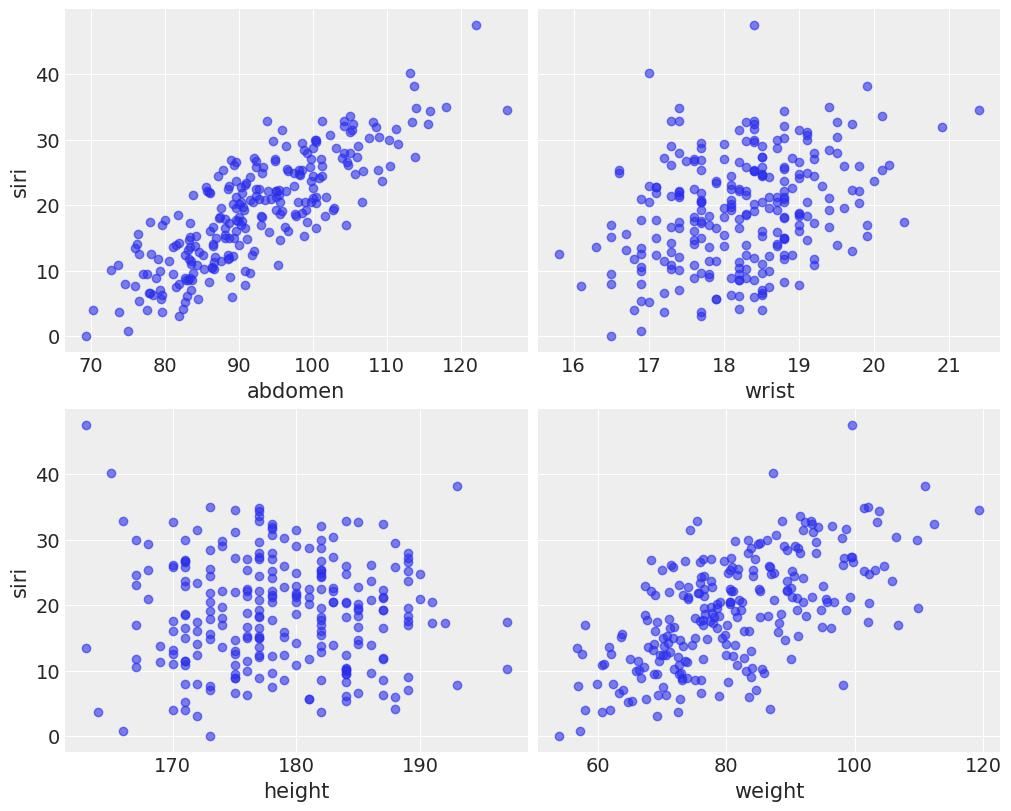
\includegraphics[width=0.85\textwidth]{Figures/1.jpeg}
		\caption{Scatter plots showing how \texttt{siri} varies with different body metrics.}
		\label{fig:siri_scatterplots}
	\end{figure}
	
	\subsection{Model Building}
	All models that we are testing are simple linear regression models where the response variable is \texttt{siri} and the independent covariates are individuals or a combination of the variables available in the dataset. We will be investigating how using a series of models and model averaging can produce improved results. All priors and linear transformations are kept simple to avoid compleximity of models. The parameters are \texttt{$\alpha$} - the intercept for the linear equation, \texttt{$\sigma$} - the standard deviation and \texttt{$\beta$} a vector of coefficients for the covariates used in the linear regression models.
	
	\subsubsection{Prior Distributions}
	\[Y \sim \mathcal{N}(\mu, \sigma^2) \]
	\[\mu = \alpha + \beta X\]
	\[\alpha \sim \mathcal{N}(0, 1)  \quad \text{with } \sigma > 0\]
	\[\beta \sim \mathcal{N}(0, 1)\]
	\[\sigma \sim \mathcal{N}(0, 5)\]
	
	Here, $\alpha$ and $\beta$ are given standard normal priors with a mean of 1 and a variance of 1 for both. The standard deviation of the residuals, $\sigma$, is also assigned a normal prior with the constraint of being positive only and the variance of 5.
	
	\subsubsection{Models and their covariates}
	
	Model 0 is defined with only the covariate \texttt{abdomen}. Model 1 is defined with the covariates \texttt{wrist}, \texttt{height} and \texttt{weight}.
	
	\subsubsection{Model Posteriors and Comparisons}
	Figure \ref{fig:model0_results} and \ref{fig:model1_results} shows posterior predictive against the sample data. In Model 0 seems to be performing worse when compared to Model 1.  In Table \ref{tab:model_comparison} we can see the ELPD scores for each model alongside with their respective weights. Based on their respective posterior predictive plots, the lower weight for Model 0 seems evident. Figure \ref{fig:model_comparison} shows all of posterior means together for all three models including the average model. While comparing , we can see that the average model is basically passing between the two models. 
	
	\begin{figure}[h!]
		\centering
		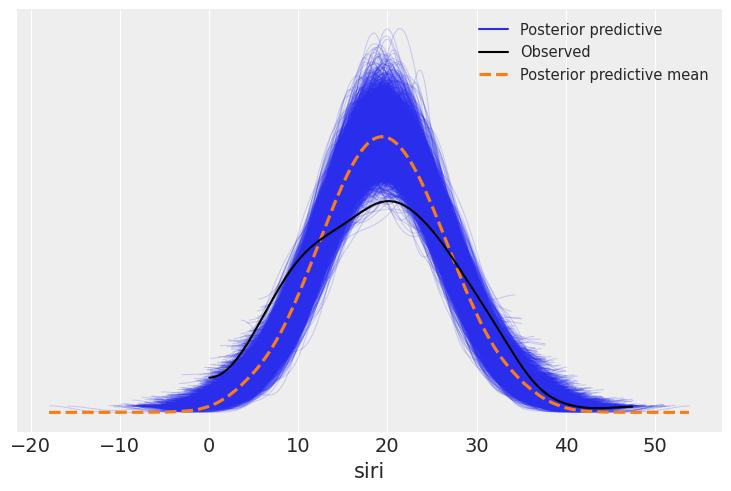
\includegraphics[width=0.8\textwidth]{Figures/2.jpeg}
		\caption{Comparison between observed distribution of \texttt{siri} and posterior predictive samples for Model-0}
		\label{fig:model0_results}
	\end{figure}
	
	\begin{figure}[h!]
		\centering
		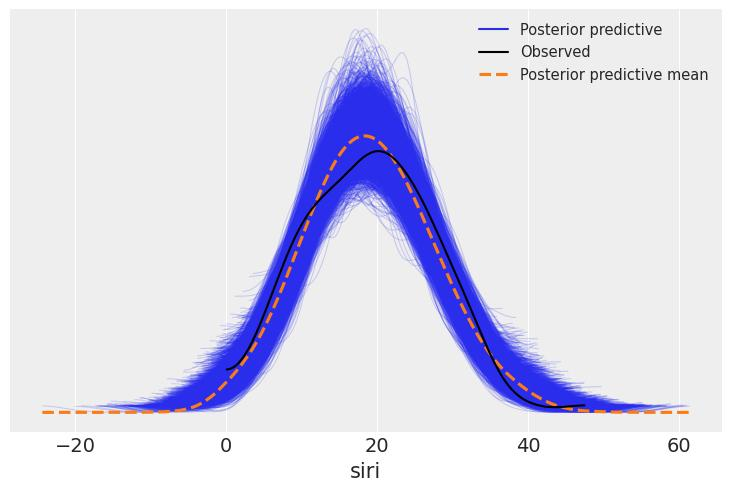
\includegraphics[width=0.8\textwidth]{Figures/3.jpeg}
		\caption{Comparison between observed distribution of \texttt{siri} and posterior predictive samples for Model-1}
		
		\label{fig:model1_results}
	\end{figure}
	
	\begin{table}[h!]
		\centering 
		\begin{tabular}{|l|r|r|r|r|r|r|r|r|}
			\hline
			\textbf{Model} & \textbf{rank} & \textbf{elpd\_loo} & \textbf{p\_loo} & \textbf{elpd\_diff} & \textbf{weight} & \textbf{se} & \textbf{dse} & \textbf{warning} \\
			\hline
			model\_1 & 0 & -817.30 & 3.70 & 0.00 & 0.64 & 10.46 & 0.00 & False \\ \hline
			model\_0 & 1 & -825.36 & 1.88 & 8.05 & 0.36 & 9.98  & 8.66 & False \\
			\hline 
		\end{tabular}
		\caption{Comparison of models using Leave-One-Out cross-validation metrics.}
		
		\label{tab:model_comparison}
	\end{table} 
		
	\begin{figure}[h!]
		\centering
		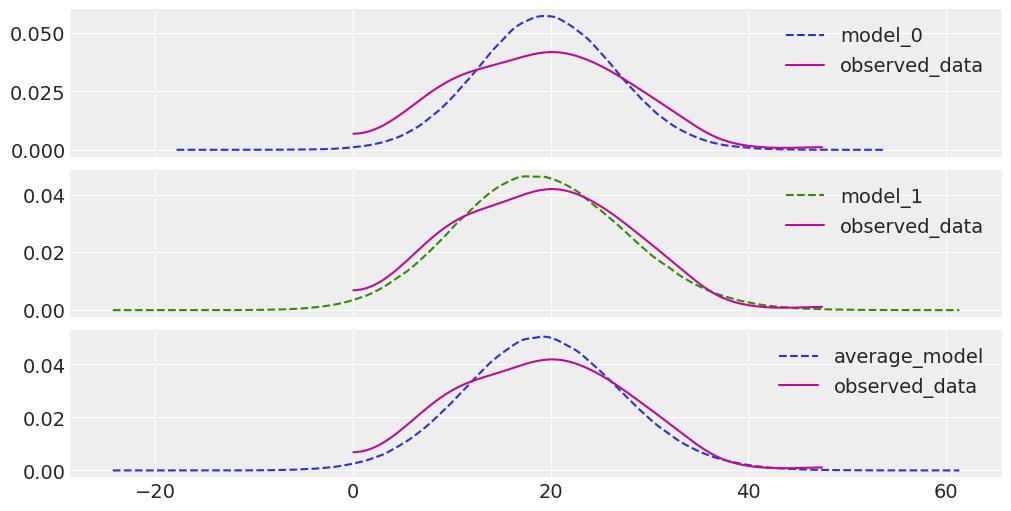
\includegraphics[width=0.9\textwidth]{Figures/4.jpeg}
		\caption{Comparison of model predictions with observed data using posterior predictive distributions.}
		
		\label{fig:model_comparison}
	\end{figure}
	
	
	
	\section{Summary}
	
	Bayesian Model Averaging (BMA) is a sophisticated approach to inference and prediction that uniquely addresses the fundamental uncertainty inherent in model selection. Instead of committing to a single "best" model, BMA operates on the idea that the true data-generating process is probably represented by a combination of probable models.
	
	BMA achieves this by constructing a weighted average of the predictions made by a set of candidate models. The weights are determined by the posterior model probabilities—a measure of each model's certainty given the observed data and prior beliefs. This results in predictions that are more robust and provide a more accurate quantification of predictive uncertainty compared to predictions derived from any single model.
	
	Although BMA is a mathematically elegant and a theoretically sound technique, its practical application faces strict requirements. It performs optimally under M-closed cases (where the true model is assumed to be in the candidate set), and its performance can degrade otherwise. Furthermore, the wider adoption of BMA is often hampered by the lack of streamlined industry standards and consensus on implementation. Nonetheless, BMA can achieve excellent predictive performance, provided the researcher makes a proper choice of a diverse set of candidate models that collectively capture unique and relevant aspects of the dataset.
	
	\newpage
	\addcontentsline{toc}{section}{Bibliography}
	\renewcommand\refname{Bibliography} 
	\bibliographystyle{plainnat}
	\bibliography{references}
	
	\end{document}